\def\mySecNum{2.3}
\mySection{\mySecNum~Put options}
%-------------- start slide -------------------------------%{{{ 1
\begin{frame}[fragile]
	\begin{center}
		Call option	: \textcolor{magenta}{Buyer} can walk away.

		\bigskip
		\mySeparateLine
		\bigskip

		???? option : \textcolor{cyan}{Seller} can walk away.
	\end{center}
\end{frame}
%-------------- end slide -------------------------------%}}}
%-------------- start slide -------------------------------%{{{ 1
\begin{frame}[fragile,t]

	\begin{mydefinition}
		A \textcolor{magenta}{put option} gives the owner the right but not the obligation to sell the
		underlying asset at a predetermined price during a predetermined time period.
	\end{mydefinition}
	\bigskip

	\begin{remark}
		Similar to the call option case, a premium paid by the put buyer at the time the option is
		purchased is needed in order to compensate the put seller for being in a disadvantage position.
	\end{remark}
	\bigskip

	\begin{center}
		\renewcommand{\arraystretch}{1.2}
		\begin{tabular}{|c|c|cc|}
			\hline
			... of put option & someone needs to &                     & premium \\ \hline
			seller            & buy              & has to buy if asked & receive \\
			buyer             & sell             & can walk away       & pay     \\
			\hline
		\end{tabular}
	\end{center}
\end{frame}
%-------------- end slide -------------------------------%}}}
%-------------- start slide -------------------------------%{{{ 1
\begin{frame}[fragile,t]
	\begin{align*}
		\text{\textcolor{magenta}{Payoff} of purchased put} & = \max \left( 0,  \text{strike price} - \text{spot price at expiration}\right) \\[1em]
		\text{\textcolor{cyan}{Profit} of purchased put}    & = \text{\textcolor{magenta}{payoff} of purchased put}                          \\
                                                        & \quad -\text{future value of option premium}
	\end{align*}
	\bigskip
	\mySeparateLine
	\bigskip
	\begin{align*}
		\text{\textcolor{magenta}{Payoff} of written put} & = - \max \left( 0,  \text{strike price} - \text{spot price at expiration} \right) \\[1em]
		\text{\textcolor{cyan}{Profit} of written put}    & = \text{\textcolor{magenta}{payoff} of written put}                               \\
                                                      & \quad + \text{future value of option premium}
	\end{align*}
\end{frame}
%-------------- end slide -------------------------------%}}}
%-------------- start slide -------------------------------%{{{ 1
\begin{frame}[fragile,t]
	\begin{myexample}
		 S\&R Index 6-month European put option
		 \begin{align*}
			 \text{Strike price}           & = \$1,000, \\
			 \text{Premium}                & = \$74.20, \\
			 \text{6-month risk-free rate} & = 2\%.
		 \end{align*}
		 Compute both payoff and profit of the \textcolor{alert}{purchased} put option if the index
		 value in six months $\textcolor{magenta}{\$1,100}$ (resp.  $\textcolor{cyan}{\$900}$).
	\end{myexample}
	\bigskip
	\pause
	\begin{mysol}\phantom{a}\\[1em]

	 \begin{minipage}{0.48\textwidth}
		\begin{center}
			If index value in six months = \textcolor{magenta}{\$1,100},
			\begin{align*}
				\text{Payoff} & = \max ( 0, \$1,000 - \textcolor{magenta}{\$1,100}) \\
                      & = \$0                                               \\
				\text{Profit} & = \$0 - \$74.20 \times 1.02                         \\
                      & = - \$75.68.
			\end{align*}
		\end{center}
	 \end{minipage}
	 \hfill \pause
	 \begin{minipage}{0.48\textwidth}
		\begin{center}
			If index value in six months = \textcolor{cyan}{\$900},
			\begin{align*}
				\text{Payoff} & = \max ( 0, \$1,000 - \textcolor{cyan}{\$900} ) \\
                      & = \$100                                           \\
				\text{Profit} & = \$100 - \$74.20 \times 1.02                     \\
                      & = \$24.32.
			\end{align*}
		\end{center}
	 \end{minipage}

	 \myEnd
	\end{mysol}
\end{frame}
%-------------- end slide -------------------------------%}}}
%-------------- start slide -------------------------------%{{{ 1
\begin{frame}[fragile]
\begin{center}
	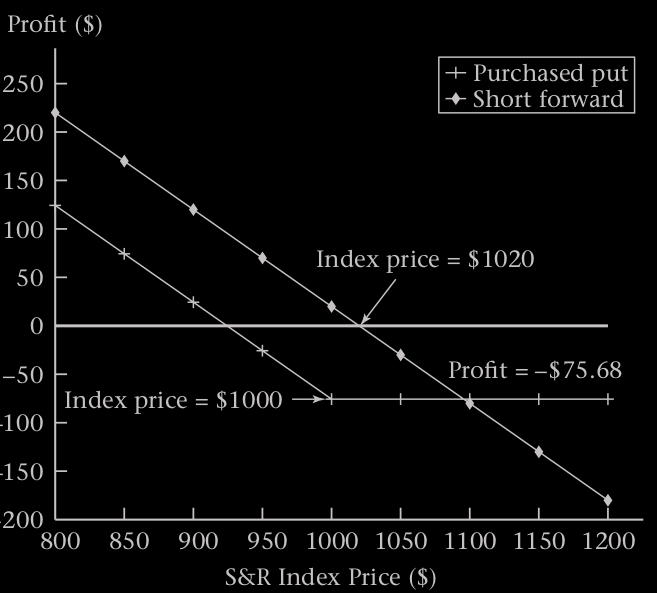
\includegraphics[scale=0.2]{figs/Figure-2-8.png}
\end{center}
\end{frame}
%-------------- end slide -------------------------------%}}}
%-------------- start slide -------------------------------%{{{ 1
\begin{frame}[fragile,t]
	\begin{myexample}
		 S\&R Index 6-month European put option
		 \begin{align*}
			 \text{Strike price}           & = \$1,000, \\
			 \text{Premium}                & = \$74.20, \\
			 \text{6-month risk-free rate} & = 2\%.
		 \end{align*}
		 Compute both payoff and profit of the \textcolor{alert}{written} put option if the index
		 value in six months $\textcolor{magenta}{\$1,100}$ (resp.  $\textcolor{cyan}{\$900}$).
	\end{myexample}
	\bigskip
	\pause
	\begin{mysol}\phantom{a}\\[1em]

	 \begin{minipage}{0.48\textwidth}
		\begin{center}
			If index value in six months = \textcolor{magenta}{\$1,100},
			\begin{align*}
				\text{Payoff} & = - \max ( 0, \$1,000 - \textcolor{magenta}{\$1,100}) \\
                      & = \$0                                                 \\
				\text{Profit} & = \$0 + \$74.20 \times 1.02                           \\
                      & = \$75.68.
			\end{align*}
		\end{center}
	 \end{minipage}
	 \hfill \pause
	 \begin{minipage}{0.48\textwidth}
		\begin{center}
			If index value in six months = \textcolor{cyan}{\$900},
			\begin{align*}
				\text{Payoff} & = - \max ( 0, \$1,000 - \textcolor{cyan}{\$900} ) \\
                      & = - \$100                                         \\
				\text{Profit} & = - \$100 + \$74.20 \times 1.02                   \\
                      & = - \$24.32.
			\end{align*}
		\end{center}
	 \end{minipage}

	 \myEnd
	\end{mysol}
\end{frame}
%-------------- end slide -------------------------------%}}}
%-------------- start slide -------------------------------%{{{ 1
\begin{frame}[fragile]
\begin{center}
	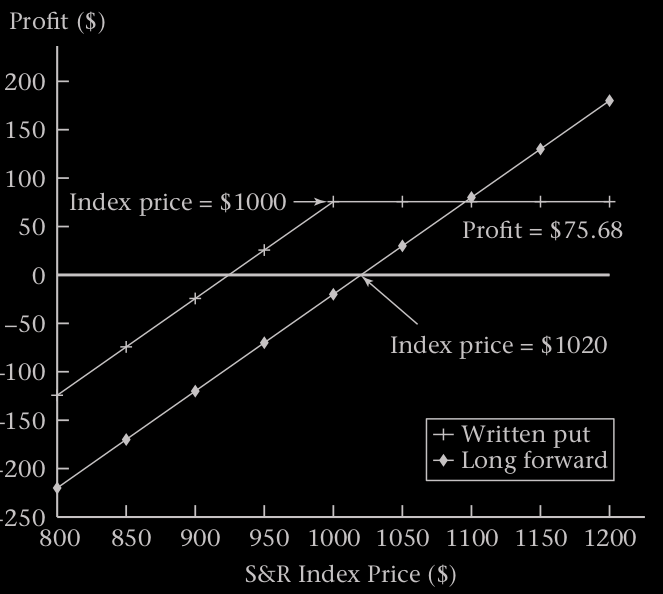
\includegraphics[scale=0.2]{figs/Figure-2-9.png}
\end{center}
\end{frame}
%-------------- end slide -------------------------------%}}}
%-------------- start slide -------------------------------%{{{ 1
\begin{frame}[fragile]
	\begin{center}
		A \textcolor{magenta}{call} option becomes more profitable \\
		when the underlying asset                                  \\
		\textcolor{magenta}{appreciates} in value

		\bigskip
		\mySeparateLine
		\bigskip

		A \textcolor{cyan}{put} option becomes more profitable     \\
		when the underlying asset                                  \\
		\textcolor{cyan}{depreciates} in value
	\end{center}
\end{frame}
%-------------- end slide -------------------------------%}}}
%-------------- start slide -------------------------------%{{{ 1
\begin{frame}[fragile,t]
	\begin{mydefinition}
		\textcolor{magenta}{Moneyness} of an option describes whether the option payoff would be
		positive if the option were exercised immediately.
		\bigskip

		In particular, one has
		\bigskip

		\begin{center}
			\renewcommand{\arraystretch}{1.2}
			\begin{tabular}{|c|c|}
				\hline
				Moneyness                                    & payoff if exercised immediately \\ \hline
				\textcolor{magenta}{In-the-money option}     & $>0$                            \\
				\textcolor{magenta}{At-the-money option}     & $=0$                            \\
				\textcolor{magenta}{Out-of-the money option} & $<0$                            \\ \hline
			\end{tabular}
		\end{center}
	\end{mydefinition}
\end{frame}
%-------------- end slide -------------------------------%}}}
